%%
%% This is file `sample-manuscript.tex',
%% generated with the docstrip utility.
%%
%% The original source files were:
%%
%% samples.dtx  (with options: `manuscript')
%% 
%% IMPORTANT NOTICE:
%% 
%% For the copyright see the source file.
%% 
%% Any modified versions of this file must be renamed
%% with new filenames distinct from sample-manuscript.tex.
%% 
%% For distribution of the original source see the terms
%% for copying and modification in the file samples.dtx.
%% 
%% This generated file may be distributed as long as the
%% original source files, as listed above, are part of the
%% same distribution. (The sources need not necessarily be
%% in the same archive or directory.)
%%
%% Commands for TeXCount
%TC:macro \cite [option:text,text]
%TC:macro \citep [option:text,text]
%TC:macro \citet [option:text,text]
%TC:envir table 0 1
%TC:envir table* 0 1
%TC:envir tabular [ignore] word
%TC:envir displaymath 0 word
%TC:envir math 0 word
%TC:envir comment 0 0
%%
%%
%% The first command in your LaTeX source must be the \documentclass command.

% Package for Coding Formatting
\documentclass[manuscript,screen,review,sigconf]{acmart}
\usepackage{listings}

%%
%% \BibTeX command to typeset BibTeX logo in the docs
\AtBeginDocument{%
  \providecommand\BibTeX{{%
    \normalfont B\kern-0.5em{\scshape i\kern-0.25em b}\kern-0.8em\TeX}}}

%% Rights management information.  This information is sent to you
%% when you complete the rights form.  These commands have SAMPLE
%% values in them; it is your responsibility as an author to replace
%% the commands and values with those provided to you when you
%% complete the rights form.
% \setcopyright{acmlicensed}
% \copyrightyear{2018}
% \acmYear{2023}
% \acmDOI{XXXXXXX.XXXXXXX}


%%
%% Submission ID.
%% Use this when submitting an article to a sponsored event. You'll
%% receive a unique submission ID from the organizers
%% of the event, and this ID should be used as the parameter to this command.
%%\acmSubmissionID{123-A56-BU3}

%%
%% For managing citations, it is recommended to use bibliography
%% files in BibTeX format.
%%
%% You can then either use BibTeX with the ACM-Reference-Format style,
%% or BibLaTeX with the acmnumeric or acmauthoryear sytles, that include
%% support for advanced citation of software artefact from the
%% biblatex-software package, also separately available on CTAN.
%%
%% Look at the sample-*-biblatex.tex files for templates showcasing
%% the biblatex styles.
%%

%%
%% The majority of ACM publications use numbered citations and
%% references.  The command \citestyle{authoryear} switches to the
%% "author year" style.
%%
%% If you are preparing content for an event
%% sponsored by ACM SIGGRAPH, you must use the "author year" style of
%% citations and references.
%% Uncommenting
%% the next command will enable that style.
%%\citestyle{acmauthoryear}

%%
%% end of the preamble, start of the body of the document source.
\begin{document}

%%
%% The "title" command has an optional parameter,
%% allowing the author to define a "short title" to be used in page headers.
\title{Can Large Language Models Generated Code That Can Compete With Model, Human-Written Code}

%%
%% The "author" command and its associated commands are used to define
%% the authors and their affiliations.
%% Of note is the shared affiliation of the first two authors, and the
%% "authornote" and "authornotemark" commands
%% used to denote shared contribution to the research.
\author{Thomas D. Chambers}
\email{tc262389@falmouth.ac.uk}
\affiliation{%
  \institution{Falmouth University}
  \city{Penryn}
  \state{Cornwall}
  \country{United Kingdom}
  \postcode{TR10 9FE}\\
  \url{https://github.com/ThomasChambers15243/Dissertation}
}

%%
%% By default, the full list of authors will be used in the page
%% headers. Often, this list is too long, and will overlap
%% other information printed in the page headers. This command allows
%% the author to define a more concise list
%% of authors' names for this purpose.




%%
%% The code below is generated by the tool at http://dl.acm.org/ccs.cfm.
%% Please copy and paste the code instead of the example below.
%%
\begin{CCSXML}
<ccs2012>
   <concept>
       <concept_id>10011007.10011006.10011073</concept_id>
       <concept_desc>Software and its engineering~Software maintenance tools</concept_desc>
       <concept_significance>500</concept_significance>
       </concept>
 </ccs2012>
\end{CCSXML}

\ccsdesc[500]{Software and its engineering~Software maintenance tools}

%\ccsdesc[500]{Do Not Use This Code~Generate the Correct Terms for Your Paper}
%\ccsdesc[300]{Do Not Use This Code~Generate the Correct Terms for Your Paper}
%\ccsdesc{Do Not Use This Code~Generate the Correct Terms for Your Paper}
%\ccsdesc[100]{Do Not Use This Code~Generate the Correct Terms for Your Paper}

%%
%% Keywords. The author(s) should pick words that accurately describe
%% the work being presented. Separate the keywords with commas.
%\keywords{Do, Not, Us, This, Code, Put, the, Correct, Terms, for,
  %Your, Paper}

\received{15 October 2023}

%%
\begin{abstract}
    Large language Models have never been more prominent than they are today, finding use in social media, essay writing, shopper predictions, investing and now software development. This paper will outline the history of code generation, LLM, and code analysis and will then attempt to investigate the practicality of LLM-generating code for software developers to use. The paper will finish off with some discussion about ethical and practical issues with code generation in general.
\end{abstract}

%% This command processes the author and affiliation and title
%% information and builds the first part of the formatted document.
\maketitle


\section{Introduction}
% What is the study in a few words
This study will investigate the practicality of using large-language models to generate Python code. These models take in a human-written prompt to generate an output, the output attempting to fulfil the desired task of the prompt through code. Within the last few years, these models have been used to generate code in many programming languages, straight into a programmer's IDE. With many large tech companies investing in generative models, such as Google and META \cite{Google_AI_2023, Meta_2023}, and bespoke versions of these models being used commercially for code productivity, such as Github's Copilot and Sourcery \cite{GitHub_2021, Sourcery_2023}, their use by programmers is rapidly increasing. %%HERE CHANGE BLACK BOX%%
LLM are often described as a black box \cite{blackBoxNature}, this describes how the user can input data and receive a response, without an understanding of the internals. This form of abstraction is very common within programming, however, where LLM stand out is that the engineers behind them also do not know. Because the internal 'synapses' of the neural network are automatically arranged by the model itself, it's extremely difficult for an engineer to decipher.
Due to this black box behaviour, an intimate understanding of how these code snippets are generated is unknown, and there's a risk that poorly written, buggy and insecure code could be used by novice and experienced programmers alike. The need to understand the level of quality of outputs is paramount before these generation tools become widespread in education and industry, so the consequences can be best understood \cite{xai}. The focus of this study will be on Open-AI's GPT models due to their API, success and public prominence.

\section{Understanding Code Generation}
% History of Code Generation
Code generation is not new, being used in many computing processes already, perhaps most well-known is the use in compilers to produce code optimisation and executable machine code. Furthermore, code generation from a human prompt has been discussed for over 50 years. PROW \cite{PROW} was an early code generation tool that could produce Perl code from an input written in predicate calculus. However, as discussed two years later by Manna and Waldinger \cite{Program_Syn}, "programmers might find such a language lacking in readability and conciseness." They went on to predict a future program synthesizer; one that works with the programmer to produce segments of code that can be incorporated into the program. They argue it would be a "more practical system" with greater "power".

% Public release of ChatGPT has blown up popularity
Fifty years later in 2022, with the public release of ChatGPT \cite{ChatRel}, public awareness of LLM significantly increased due to the wide adaption of its chat feature. Generation models have been used for years to write essays, generate art and synthesise an actor's voice, the implications of such have caused many to re-evaluate the current state and future of educational and business environments \cite{GPTBusinessImpact, GPTEducationImpact, ethicalImpact, LaborMarketImpact}, but more recently the use of generation has become more relevant in a programmer's workflow.

% Generated code evolution up to codex then CoPilot
\subsection{The Background of LLM}
% How do LLM work roughly (not super important for this paper but it does need to be in here. Almost all papers leave it out as assumed knowledge so just a quick overview is sufficient)
The rising popularity of LLM generation is in-large due to their apparent success at task completion, giving them the appearance of being \textit{intelligent}. However, by any definition today, at most it's pseudo-intelligence. This section will first give a very brief overview of the workings of LLM, why they're pseudo-intellectual and then their current use today.

Large language models are neural networks trained to predict the next token in a sequence, the token, in the case of code generation, being characters in a string.
\[P(Token_n|Token_1,Token_2,...,Token_{n-1})\]
GPT stands for \textbf{G}enerative \textbf{P}re-trained \textbf{T}ransformer. The generation means that it can predict the next token, pre-trained means that the model has received a large amount of data and has had its bias adjusted and a transformer is an encoder-decoder network that adds \textit{self-attention}. Self-attention results in significant performance increases in accurate prediction. LLM that have been pre-trained can be further \textit{fine-tuned} to improve performance at specific predictions. Although the prediction can be extremely accurate, there is no logical reasoning behind the prediction that can be seen as akin to human intelligence. The accurate predictions serve to mimic human intelligence.

%%% Discussion about the studies performance of LLM tools already in use %%%

In 2021 OpenAI released their fine-tuned model GPT-3 codex, trained on 54 million public software repositories hosted on GitHub \cite{CodexRelPaper}. Released the same year \cite{GitHub_2021}, Github's CoPilot is a generation model with a heavy reliance on Codex. To test the functional performance of Codex, the team behind OpenAI released the humanEval data set. A public repository to benchmark the performance of generated code. They also implemented the technique \textit{pass@k}. An unbiased calculator to estimate the success of a model given \textit{k} samples. Functional performance is found by the ability to generate code from a prompt that successfully passes given unit tests, failures often due to syntax errors, invoking out-of-scope functions or referencing non-existent variables. Within their data set, Codex had a higher performance than all previous GPT-model, solving 70.2\% of problems with 100 samples. The functional performance of Codex and models alike have been replicated numerously \cite{SysEvaOfLLMofCode, PerformanceParsonProblems, CopilotSuggestionsEval, CoPilotForTeaching}, with Codex being able to outperform students in even CS1 questions and, although performance dropped, still compete with students in CS2 questions \cite{Codex_CS1_CS2_Test}. CS1 questions covered the basics of programming, with topics such as "variables, arithmetic, conditional branches, loops, reading and writing to files, and functions". CS2 took questions further, covering questions about hashing, discrete mathematics, OOP and ADTs. During these questions, the model could recognise algorithms by name and produce efficient solutions for those problems, such as tree or graph searches and modifications.

\subsection{Issues with the Current State of Code Generation}
 Large language models have proven to appear highly performant, however, several technical and practical limitations should be carefully understood.

\textit{Firstly}, models are not uniform across languages. Nguyen and Nadi \cite{CopilotSuggestionsEval} found that CoPilot functionally performed best when writing in Java and worst in Javascript. Other researchers have written their own fine-tuned model, Poly-Coder, based on the GPT-2 architecture, which outperforms all GPT-based models in the C language \cite{SysEvaOfLLMofCode}. Its was argued that the low score in C was possibly due to a problem with the data-set and fine-tuning process being over-reliant on Python and under focused in C.

\textit{Secondly}, the results are not \textit{one-shot}. Codex can respond with very variant accuracy in its solutions, hence why most investigations use several responses, such as with \textit{pass@k} often using 100 samples. This is not the standard programming experience; a student does not submit 100 solutions to be marked by their professor, leading to the comparison being fallacious. An attempt to control this compared students to Codex, except also gave students multiple attempts at solutions, their success frequently increases with each attempt. However, they found that Codex was still competitive with students, even after multiple submissions \cite{Codex_CS1_CS2_Test}.

\textit{Thirdly}, responses vary significantly depending on the value of the model's temperature. Temperature is a value used in neural networks to increase entropy (effectively randomness) in the softmax distribution, the distribution which controls the quality and diversity of the predictions. This affects the output layer where tokens are sampled from. A higher temperature increases how 'surprising' the next token will be \cite{temperatureSoftMaxhinton2015distilling, temperaturewang2020contextual}. Multiple studies have found that with a higher temperature, models can achieve a higher \textit{pass@k} score at larger samples, despite producing more erroneous code. Across multiple studies, researchers found optimal performance at T0.6, with T0.2 and T0.8 also performing well. Temperature and sample size were found to be proportional, this is likely due to the diversity of code at higher temperatures needing a higher sample rate to score \cite{stackOVerflowAndTemperature, SysEvaOfLLMofCode, CodexRelPaper}.

\textit{Fourthly}, there is a significant reason to question whether the success of generated code translates into actual programmer performance, even with their access becoming more streamlined. CoPilot can directly embed into your IDE, finishing off lines or blocks of code for the user. There is also a chat option in VS Code where prompts can be given and code can be directly copied into the user's file, currently in beta. However, when a programmer uses a piece of code, they have to evaluate the code before use as it might contain bugs, be a sub-optimal solution or generally poorly written. In a study of 24 participants using Copilot \cite{Expectation_vs_Experience}, they found that even though code generation gave promising results, it did not improve overall programming time or the success rate of those participants using the tool. CoPilot even led to more task failures in the medium and hard category of tasks, where programmers might have not understood the generated code or spent longer debugging the code than if they had just written it themselves. Nevertheless, 23/24 of the participants still found it more useful than Intellisense and the majority "overwhelmingly preferred using Copilot in their programming workflow since Copilot often provided a good starting point to approach the programming task." The study showed CoPilot to be an imperfect aid. It can allow a programmer to instantly generate an often feasible solution to a task, however, in doing so they remove themselves from the task of problem-solving, which often exposes the programmer to online discussion and related topics, advancing their technical skill. Other researchers have discussed this problem, hypothesising that code generation is an efficient tool for seasoned programmers, but can turn into a liability when used by novice programmers who do not fully understand the problem, context and generated solution \cite{CopilotPairProgrammer}.

\section{Quality Code}
% Importance of code analysis, reference Dijkstra, maybe clean code and Goole/Ibm
Good quality code is vital for creating maintainable software that can last, but still, there is discourse around what good quality code is. In 1969 Dijkstra wrote in a letter, \textit{"A programmer has only done a decent job when his program is flawless and not when his program is functioning properly only most of the time."} He criticized the attitude of programmers of his time, something that he saw as a \textit{"software crisis"}. He saw programmers treating debugging as a necessity, rather than what he believed, an inevitable consequence of poorly written systems. He argued that writing \textit{"intellectually manageable" programs} would reduce the amount of reasoning involved in justifying their proper operation and a reduction in the number of test cases. If done correctly, he claims that \textit{"the correctness can be shown a priori"}, so a need for zero test cases. Dijkstra laid out a fundamental argument for why quality code is necessary which has been built upon ever since \cite{EWD:EWD288}.

Recognising when code is \textit{"intellectually manageable"} is a complex issue. Greg Michaelson wrote that \textit{"Programming style is notoriously difficult to characterise"} and that imperative languages have been the \textit{"source of endless theological disputes"}, such as the use of GOTOS, the use of recursion over iteration or the number of parameters a sub-program should have \cite{Automatic_analysis}. While for the most part, experts agree on the abandonment of goto's in structured programming \cite{gotoConsideredHarmful, KnuthGoTo}, the rest are still up for debate.

The quality of generated code is vital if the produced code is ever expected to be used in a practical sense. However, the common mantra, \textit{garbage in, garbage out} is just as true now, the quality of written code largely depends on the quality of the code within the data set. Unfortunately,  the fine details of the data sets used for available LLM are kept private, \cite{SysEvaOfLLMofCode}, so to assess the quality of code, we can use code metrics as an attempt to judge the outputted code.


\subsection{Code Analysis}
% Write about different code metrics and how they've been used to measure student work
Pre-1980, software metrics generally worked as a regression model between two variables, conceptually simple, mostly relying on resources and quality. However, during the mid-late 70s, software metrics saw a new direction with Halstead and McCabe \cite{FENTON1999149}. They extracted information from the code design rather than just the static code.

Halstead developed a set of formulas that, when given a code input, would produce a series of scores based on the number of unique and total amount of operands and operators used \cite{Halstead}. The definition of Operands and Operators has slightly different meanings depending on the implementation, but generally, operators are all normal operators, keywords and brackets of all kinds ( (), [], {} ). Operands are variables, methods or function declarations and constants such as Boolean values and strings. Halstead metrics produce useful scores of the complexity of code, such as an estimate of the time to program and the potential for bugs. Although Halstead metrics are not free from critique, various definitions can cause trouble when comparing scores, the use of magic numbers (18 appearing in the Time formula) appears to be arbitrary and it can be argued that the use of operands and operators is too simplistic for modern programming.

Other code metrics take different approaches to Halstead to achieve the same goal of scoring code. The \textit{Flesch-Kincaid readability test} \cite{FleschReading} is a method to score the readability of human written language, based on the number of \textit{syllables per words} and \textit{words per sentence}, similar to how Halstead used operators and operands. Kurt Starsinic developed a module, \textit{Fathom.pm}, to apply the Fleshc-Kincaid test to Perl code, producing a score based on the number of \textit{{}tokens per expression}, \textit{expressions per statement} and \textit{statements per subroutine} \cite{Starsinic_1998}.
\\ \\
Code Complexity =\\
  ((average expression length in tokens) * 0.55)\\
+ ((average statement length in expressions) * 0.28)\\
+ ((average subroutine length in statements) * 0.08)\\
\\
The formula would produce a score from 1 - 7, where 5 is "Trival" and 7 is "Very Hairy".  However, he did not provide any justification for the weights used in the formula except that they were fined-tuned through trial and error.
Börstler, Caspersen and Nordström would later produce a similar metric method to Starsinic, while also using the FLesch-Kincaid test. They introduced the Software Readability Ease Score (SRES) by treating the "lexemes of a programming language as syllables, its statements as words, and its units of abstraction as sentences" \cite{borstler2007beauty}. They argued that this type of static code analysis was a clear indicator of how readable, and thus maintainable the code was. However, to quote Dijkstra, other factors affect the "\textit{goodness}" of code, such as control flow.

In 1976, McCabe proposed a technique called \textit{Cyclomatic complexity} for scoring the control flow a program takes \cite{A_Complexity_Measure}. This was an attempt to "\textit{provide a quantitative basis for modularization}" as a way to identify in advance modules which will be difficult to maintain. McCabe provides the definition
"\textbf{Definition 1:} \textit{The cyclomatic number V(G) of a graph G
with n vertices, e edges, and p connected components is}

\[v(G)=e- n+p\]
\\
Cyclomatic complexity can be viewed as building up graphs from smaller components, examples of which McCabe included.
\begin{figure}[h]
    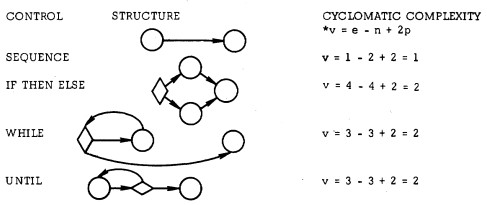
\includegraphics[width=8cm]{controlFlowDia.jpg}
    \caption{Generated Control Structure Graphs \cite{A_Complexity_Measure}}
    \label{fig:CC Graphs}
    \centering
\end{figure}

However, Cyclomatic complexity does not handle all the intricacies of code, especially since it does not consider else, do \& try, object creation and method calls. Furthermore, there are different interpretations of the method, with some researchers testing complexity at only a module level, while others at a program level, summing up the scores of individual modules. This inconsistency disrupts the comparison of results \cite{McCabeCritique, NoviceCodeWriting}.  While none of these metrics are perfect estimates of complexity, they allow for fast, accurate judgment of code. Halstead and McCabe developed their metrics during an era of batch programming where systems were significantly smaller today. While they may be ill-suited for large, industrial software, this makes them the perfect solution to measuring smaller, generated code pieces which inherently lack the complexity in which these metrics can not accurately judge \cite{metricCritique}.

% Talk about how there is a gap in the research when it comes to the analysis of generated code
To accurately ascertain a meaningful judgement of code quality, several measurements must be taken that account for the complexity of each line \textit{and} the path the code can take throughout the program. This approach of using code metrics to judge LLM generation is sparse in the current field of research \cite{CopilotPairProgrammer, CopilotSuggestionsEval}, with researchers focusing on functional performance. The practicality of code generation relies in large part on the maintainability of the code, not just its functional performance, and requires better understanding.

\section{The Research}
% Research Question & Hypothesis
\textbf{RQ:} Can large language models generate code for small-scale problems that compete with model, human-written answers.\\\\
\textbf{Null Hypothesis \(H_0\):} Large language models can generate code for small-scale coding problems that produce equal scoring in a range of given metrics when compared to model, human answers.\\\\
\textbf{Alternative Hypothesis \(H_1\)} Large language models can generate code for small-scale coding problems that produce higher scoring in a range of given metrics when compared to model, human answers.

\subsection{Research Methods}
% Philosophical Position of a positivist ontological position
My research will be grounded in a positivist ontological stance, attempting to gather an objective view of performance that can be replicated consistently elsewhere, supported by a sound methodology and statistical analysis.
For the study, GPT3.5 will be tasked with solving 20 questions of varying difficulty. GPT3.5 has been chosen due to its current widespread use and ease of access. GPT's functional performance will be measured using \textit{pass@k} and its ability to produce quality code will be measured using two metric scores, Halstead and cyclomatic complexity. Halstead metrics will allow a comparable overview of generations and the model's ability to consistently write clean code. Cyclomatic complexity will focus on the structure of said code, providing insight into maintainability. This two-pronged approach will give an overview of the models practically.
If the model can produce code that scores higher than the model answers' scores, then the \(H_1\) will be accepted - GPT is competitive.

% Research Method (Sampling/Measurements/Experimental Design)
All data pre-analysis will be in the form of floats. Several samples will be taken at different temperatures at different sample rates. Temperatures will range from T = 0.3 - 0.9 and sample sizes will range from k = 10 - 100. This is following what OpenAI's team has done with the \textit{pass@k} metric so that my data is easily comparable with theirs and other researchers in the field. Nine groups of data will be produced from this, each with the answers to each question in the set. The size of each group will be different depending on the sample rate.

\begin{table}[H]
    \centering
    \begin{tabular}{c|c|c|c}
        0 & T = 0.3 & T = 0.6 & T = 0.9\\
        \hline
        k = 10 & G13 & G16 & G19\\
        k = 50 & G53 & G56 & G59\\
        k = 100 & G103 & G106 & G109\\
    \end{tabular}
    \caption{Groups of Samples}
    \label{tab:sampleGroups}
    \vspace{-10mm}
\end{table}

For example, G32 will have \(20 * 100 -> 2,000\) generations while G19 will have \(20 * 10 -> 200\) generations. The generations will be evaluated for functional performance, this will allow me to gauge the difficulty of the questions for reflection on the study. The groups will then be combined, to form 20 groups, one per question, with 480 generations each, 9,600 in total. Lexical analysis will extract tokens for calculating the Halstead and Cyclomatic Complexity per generation. These will be summed and averaged for each question, producing one mean value per question.

\subsection{Hypothesis Testing}
To test the null hypotheses, I will be using an independent samples 1-tailed t-Test to compare the GPT and human groups. This test is a parametric test that compares whether there is a statistically significant difference between the two groups' means.

The independent variables will be the two groups, the collection of GPT generations and human answers. The dependent variable will be the metric score and each sample will be a question. In total, 20 samples per group. The data for each sample will be numerically continuous, ratio values. Before the t-test, a f-test will be evaluated to check the homogeneity of variances and a Shapiro test to ensure the data is normally distributed. The R code for the t-Test is shown below, with \textit{testData} as the given example data set. The full R code can be seen in the linked repository.

% Update once Joe's answers are here
\subsection{Pilot Study}
% Update section to involve analysis against Joe's answers.
A pilot study, which is already taking place, uses only 6 simple programming questions. Code is generated for all 6 using the same temperature, 0.6, and are being tested against Halstead metrics. Throughout this, it found that GPT produces competitive code against model answers for these simple problems, aligning with results from other research \cite{Codex_CS1_CS2_Test}. Informed by this, only medium to difficult questions will be used. An example of one of these pilot problems, as it was given in prompt form, is shown below, along with one of the generated responses. The complete set of questions is viewable in appendix section .1.
\\ \\
\textbf{Problem 2}: \textit{Given a string s containing just the characters '(', ')', '{', '}', ' [' and ']', determine if the input string is valid. An input string is valid if: Open brackets must be closed by the same type of brackets. Open brackets must be closed in the correct order. Every close bracket has a corresponding open bracket of the same type. Return a Boolean Value. Name the function P2}


\textbf{Generated Solution, T = 0.6} - (\textit{mapping has been renamed to m for spacing})
\begin{lstlisting}[language=Python]
def P2(s):
 stack = []
 m = {')': '(', '}': '{', ']': '['}
 for char in s:
   if char in m:
       if not stack or stack.pop() != m[char]:
           return False
   else:
       stack.append(char)
 return not stack
\end{lstlisting}


\begin{table}[H]
    \centering
    \begin{tabular}{|c|c|c|} \hline
         \textbf{Halstead Metric} & Generated Answer & Human Answer\\
         \hline
         Temperature & 0.6 & 0.0 \\
         Distinct Operators & 18.0 & 0.0\\
         Distinct Operands & 15.0 & 0.0\\
         Total Operators & 41.0 & 0.0\\
         Total Operands & 27.0 & 0.0\\
         Vocabulary & 33.0 & 0.0\\
         Length & 68.0 & 0.0\\
         Estim Prog Len & 133.66 & 0.0 \\
         Volume &  343.02 & 0.0\\
         Difficulty &  16.2 & 0.0\\
         Effort & 5556.9 & 0.0\\
         Time &  308.72 & 0.0\\
         Estim Bugs & 0.11 & 0.0\\
         \hline
    \end{tabular}
    \caption{Problem 2: Table of Halstead Scores for Human and generated code}
    \label{tab:HalsteadMetrics}
\end{table}

%% Compare to Joe here, replace p1,p2,p3,p4,p5 with just Joe's solutions and generated solutions to p1,p2
Table 2 shows the calculated Halstead scores for generated solutions to problems p1-p5.

% Ethical Considerations (Joe as a collaborator, no participants)
\subsection{Ethical Considerations}
As the nature of this research is a desk-based experiment, there is no need for participants. For the human-written answers to problems, I will be carefully constructing answers which abide by commonly accepted coding standards, rather than sourcing the answers from participants. Using an LLM runs the risk of the model producing code that matches private code in its training data, however, not only is matching code extremely rare for GPT models ("< 0.1\%") \cite{CodexRelPaper}, all training data is public access which is exempt from copyright under research use \cite{ExceptionToCopyright}.

For the pilot study, I had one collaborator, Joseph Walton-Rivers, a lecturer at Falmouth University. He provided the human-written code solutions for the pilot study's comparison. No personal data was collected about him or his submissions and the code was collected before the pilot study began, he had no involvement or responsibilities during the study. In answers can be viewed in the appendix section .2. %UPDATE WHEN ANSWERS ARE ACUALLY THERE%

\section{Artefact}
% Rich Description
The artefact for this project will be a combination of several components, code generation, response testing and metric gathering, all combined in one pipeline streamlining the research.
\begin{itemize}
    \item Generation\\
    Each question will have a response generated using OpenAIs API, using the GPT-3.5 turbo model. Each question can be sent \textit{k} number of times, depending on the desired sample rate, temperature can also be varied per request from 0.3 - 0.9. While prompt engineering can almost guarantee only valid code is returned, some cleaning of the response will have to take place to remove extra text returned, such as text explaining the code. No modification of the generated code sample will take place during the cleaning.
    \item Testing\\
    The gathered responses will written to a file and automatically run against a wide range of test cases, suited for each question, to test whether the return code can pass the question. These are examples of these in the appendix section .3.
    \item Code Analysis\\
    The generated code will be analysed through two methods, Halstead and Cyclomatic Complexity. Halstead will provide a wide range of 12 metric scores about the generated code, while cyclomatic complexity will provide a single score about the generated code's complexity. Both methods will be implemented within the artefact, according to the original algorithms as written by Halstead and McCabe, rather than being imported through an external library.
\end{itemize}

Development is already underway due to the preceding pilot study. The artefact and generated code will all be written in Python, due to the non-time-critical nature of the code, and the ease with which Python can handle API requests, file I/O and unit tests. Results of the study will be written to a csv file for all calculations, allowing for easy storage, use and transportation of data into R for further analysis..

\begin{figure}[h]
    \includegraphics[width=8cm]{finishedPipline.jpg}
    \caption{Generation to Metrics Pipeline}
    \label{fig:CC Pipeline}
    \centering
\end{figure}

\subsection{Development Lifecycle}
% Development Method (System Lifecycle)
Development will take place with an active use of version control through Github. To program the artefact, a waterfall-like approach with elements of Test Driven Development will be used. Tests for the lexer and metrics will be written before their complete implementation, to ensure the implementation is true to the original implementations. A waterfall-like approach will be taken to ensure academic integrity within the metrics and sub-sequence analysis. However, there is room for iteration upon some of the tools used, such as changing language if necessary or the lexing approach.
Unit testing will be used to ensure the lexer parses the correct amount of tokens and that the Halstead calculations and cyclomatic complexity score return the correct values.

Testing of the artefact will involve 5 types of tests,
\begin{itemize}
    \item \textbf{Unit testing} of every individual function that is necessary to ensure functionality. Carried out by unit tests
    \item \textbf{Integration Testing} to ensure that all components can function together. Carried out by a range of unit tests
    \item \textbf{Stress Testing} to ensure that the artefact can handle at least twice the maximum expected input size. To test, the software, large Python files will be run against the analyser to ensure the components, working together, can handle long input.
    \item \textbf{Acceptance Testing} to ensure that the artefact can meet the requirements of the study.
    \item \textbf{A Sanity Test} after every push to the main branch.
\end{itemize}


\section{Discussion}
% Go over some of the wider ethical implications of generative code
Within programming circles, the prevalence of generative models shows no sign of slowing down in common use; if the generation of code is shown to be practical, the implications of such must be considered.
\subsection{Plagiarism}
% Argument of Stolen Code
As previously discussed, generated code is formed through prediction. Every line of code generated is technically new since it's never directly copied and the model has no knowledge of its training data, \textit{however} all its training has come from human-written code. There is a non-zero chance it might directly replicate lines of code from its training data. This can be argued in an ethical and legal sense as plagiarism, no matter how unintentional. The current way developed circumvent this is to use open-source repositories as the data set, where coping the code is under a fair licence. This is also not an issue if the model has been fine-tuned on private company repos for in-house use, which is now a feature offered by CoPilot. However, the use of generated code is still in complete control of the user making the request, it is reasonable to view the code as akin to auto-complete, and still the user's own.
\subsection{Workload}
% Argument of programmers becoming too reliant on code
The use of generative models might also have a considerable impact on programmers' workflow and involved labour markets. As generative code becomes more and more feasible for use, the impact on a programmer's workload is uncertain, but it's likely their focus will drift to their other responsibilities, such as architectural design \& analysis, integration, maintenance and client management. This could have effects on the hiring process and structure of development teams if the impact of generation is large enough. Models also import libraries at different rates, "learning" from the most common habits of their training data, displaying a bias towards \textit{mediocrity }. Most likely, this would reinforce already popular and standard imports while making it harder for newly released libraries to gain prominence.
\subsection{Security}
Programmers must be aware of their inclusion of generations due to possible security concerns within the code. The entire set of training data has not been vetted for possible vulnerabilities and erroneous generations could produce further vulnerabilities. Bad faith actors might also attempt to \textit{poison} the training data. If they can include vulnerable code in the training set, through manipulation or large creation of public repositories, LLM may bias and generate this code, exposing users to high risks.
\subsection{Education}
% Educational argument that students could pass off generated code as their work
% If the hypothesis is true, then it means the skills of programmers and the quality of computing graduates might drop.
The use of ChatGPT is already prominent in education, with significant use in essay writing, tools to discover such use, such as ChatGptZero have shown promising results but still result in many false negatives and positives. Generated code is harder to detect, since two implementations of the same algorithm are likely to be very similar to one another, as is the nature of programming. The challenges students face during their studies are often better suited for code generation, as they are smaller in scale than problems faced by \textit{real-world} software engineers. Educators face a difficult challenge in identifying when a student has written code themselves, or simply passed the problems through a model and copied the answer. Not only does this hurt the reputability of education, it affects the quality of the students learning. Reliance on generation removes the student from the difficult process of learning to program; critical thinking, implementation, debugging and research. However, it might also provide a fast starting point for students to start their research. More study is needed to evaluate the impacts of code generation in education.

\section{Conclusion}
The use of LLM is only increasing as are the possible use cases and ethical issues along with them. The best practical understanding we can achieve will help equip students, workers, researchers, educators and businesses to utilize them without exposing themselves to a wide range of issues. This research should provide insight into understanding these generations and hopefully help inform the next steps for LLM uses.

%% The acknowledgements section is defined using the "acks" environment
%% (and NOT an unnumbered section). This ensures the proper
%% identification of the section in the article metadata, and the
%% consistent spelling of the heading.
\begin{acks}
Thank you Joseph Walton-Rivers for providing the model answers in the pilot study
\end{acks}

%%
%% The next two lines define the bibliography style to be used, and
%% the bibliography file.
\bibliographystyle{ACM-Reference-Format}
\bibliography{base}

\section{Appendix}

\subsection{Six Problems Used in Pilot Study}

\textbf{P1:} You are given a non-negative floating-point number rounded to two decimal places celsius, that denotes the temperature in Celsius. You should convert Celsius into Kelvin and Fahrenheit and return it as an array ans = [kelvin, fahrenheit] Name the function P1.\\

\textbf{P2:} Given a string s containing just the characters '(', ')', '{', '}', ' [' and ']', determine if the input string is valid. An input string is valid if: Open brackets must be closed by the same type of brackets. Open brackets must be closed in the correct order. Every close bracket has a corresponding open bracket of the same type. Return a Boolean Value. Name the function P2\\

\textbf{P3:} Given a string of unknown length, find the longest, unbroken sequence of the same character. For example, “aaa” is an unbroken sequence of length 3. In the string “asdjrrrraduu”, “rrrr” is the longest sequence of length 4. Return the length. Name the function P3.\\

\textbf{P4:} Given an array of strings, remove, if any, all duplicate elements. Duplicate elements are elements in the array that are evaluated as the same, so “John” == “John” but “sam” ≠ “Sam” and “John” ≠ “Sam”. Return the length of the new array. Name the function P4.\\

\textbf{P5:} Given an unsorted array of integers, return the array in sorted order, with index 0 being the smallest and the last index being the largest in the array. Duplicates can be in either order next to each other. Name the function P5\\

\textbf{P6:} Given two arrays of strings, combine them into one sorted array, with the shortest length string at index 0 and the longest length string at the last index. If two strings are the same length, sum up each string’s characters’ ASCII value, and use that total, inserting the smallest first. Return the new array. Name the function P6.\\

\subsection{Human Written Answers to Problems}

\subsection{Example Unit Test for Generated and Human Code from The Pilot Study}
\begin{lstlisting}[language=Python]
class TestP2(unittest.TestCase):
    def test_valid_brackets(self):
        valid = ["()", "[]", "{}",
                "()[]{}", "{[()]}"]
        for i in valid:
            self.assertTrue(P2(i))
    def test_invalid_brackets(self):
        invalid = ["((","))","({","})",
                    "][","}{","({[","]})",
                    "({[)}]"]
        for i in invalid:
            self.assertFalse(P2(i))
\end{lstlisting}


\end{document}
\endinput
%%
%% End of file

Notes -
Explain black box nature
Explain what a cs1 & cs2 questions
EXPLAIN WHAT MODEL TEMPERATURE IS
Be more opinionated in the use of metrics
positivist ontological stance - Little justification
Such as non-commented comments - clarify about how gpt returns explenations
Explain why failed code will still undergo anaylsis
Change section 6 title
Expand on library imports in section 6
    Purposely fuck with training data to push malicious code
Future Works Section